\chapter{METODOLOGI}
% Ubah bagian-bagian berikut dengan isi dari desain dan implementasi

Eksperimen pada penelitian ini akan mengikuti konvensi standar eksperimen DRL sebelumnya, yaitu menguji coba dan mengevaluasi performa agen dalam \emph{environment} dengan membandingkan nilai \emph{reward} yang diterima oleh agen.
Agen akan melakukan \emph{training} dalam \emph{environment} yang telah dibuat.

\section{Perangkat}

Eksperimen dalam penelitian ini menggunakan beberapa perangkat keras dan perangkat lunak.


\subsection{Perangkat Keras}

Proses \emph{training} agen dilakukan dengan sebuah komputer. Komputer tersebut memiliki spesifikasi:
\begin{itemize}
  \item Processor: Intel I7 9700K
  \item Graphics Card: RTX 2080 SUPER
  \item RAM: 32GB DDR4
  \item SSD: 512GB NVME PCIE Gen 3
\end{itemize}

\subsection{Perangkat Lunak}

Beberapa pernagkat lunak digunakan untuk menunjang pembuatan \emph{environment} dan agen DRL dalam eksperimen ini:
\begin{itemize}
  \item Python
  \item Visual Studio Code
  \item Tensorboard
  \item Ray RLlib
  \item Pygame
  \item PettingZoo
  \item Numpy
  \item Matplotlib
\end{itemize}
\section{Desain Environment}
Desain dari \emph{environment} adalah modifikasi dari Inquisitive Otter's Civ6 environment \citep{civ6Environment}. 
Desain awal dari \emph{environment} ini hanya memiliki sebuah agen \emph{attacker} dan memiliki mekanisme yang kurang sesuai dengan mekanisme Civ6.
\emph{Environment} yang sudah dimodifikasi ini juga sudah diimplementasikan ke dalam PettingZoo.
Implementasi ke PettingZoo memudahkan untuk mengintegrasikan \emph{environment} ini dengan library RL lain.

\subsection{Area dan Posisi}
\emph{Environment} merupakan area \emph{pointy top hexagonal grid} berukuran 8x8. Di tengah area tersebut terdapat sebuah kota.
\emph{Environment} yang sudah termodifikasi memiliki dua jenis agen yaitu agen \emph{attacker} dan agen \emph{defender}.
Setiap agen memiliki 3 \emph{unit} jarak dekat (\emph{melee}) (\emph{warrior}) dan 2 \emph{unit} jarak jauh (\emph{ranged}) (\emph{slinger}).

Penempatan \emph{unit} agen dilakukan secara acak dengan pembatasan.
\emph{Unit} agen \emph{attacker} ditempatkan minimal sejauh 5 lantai dari kota di tengah area.
\emph{Unit} agen \emph{defender} berada di lantai sebelah kota.


\begin{figure}[H]
  \centering
    % Nama dari file gambar yang diinputkan
    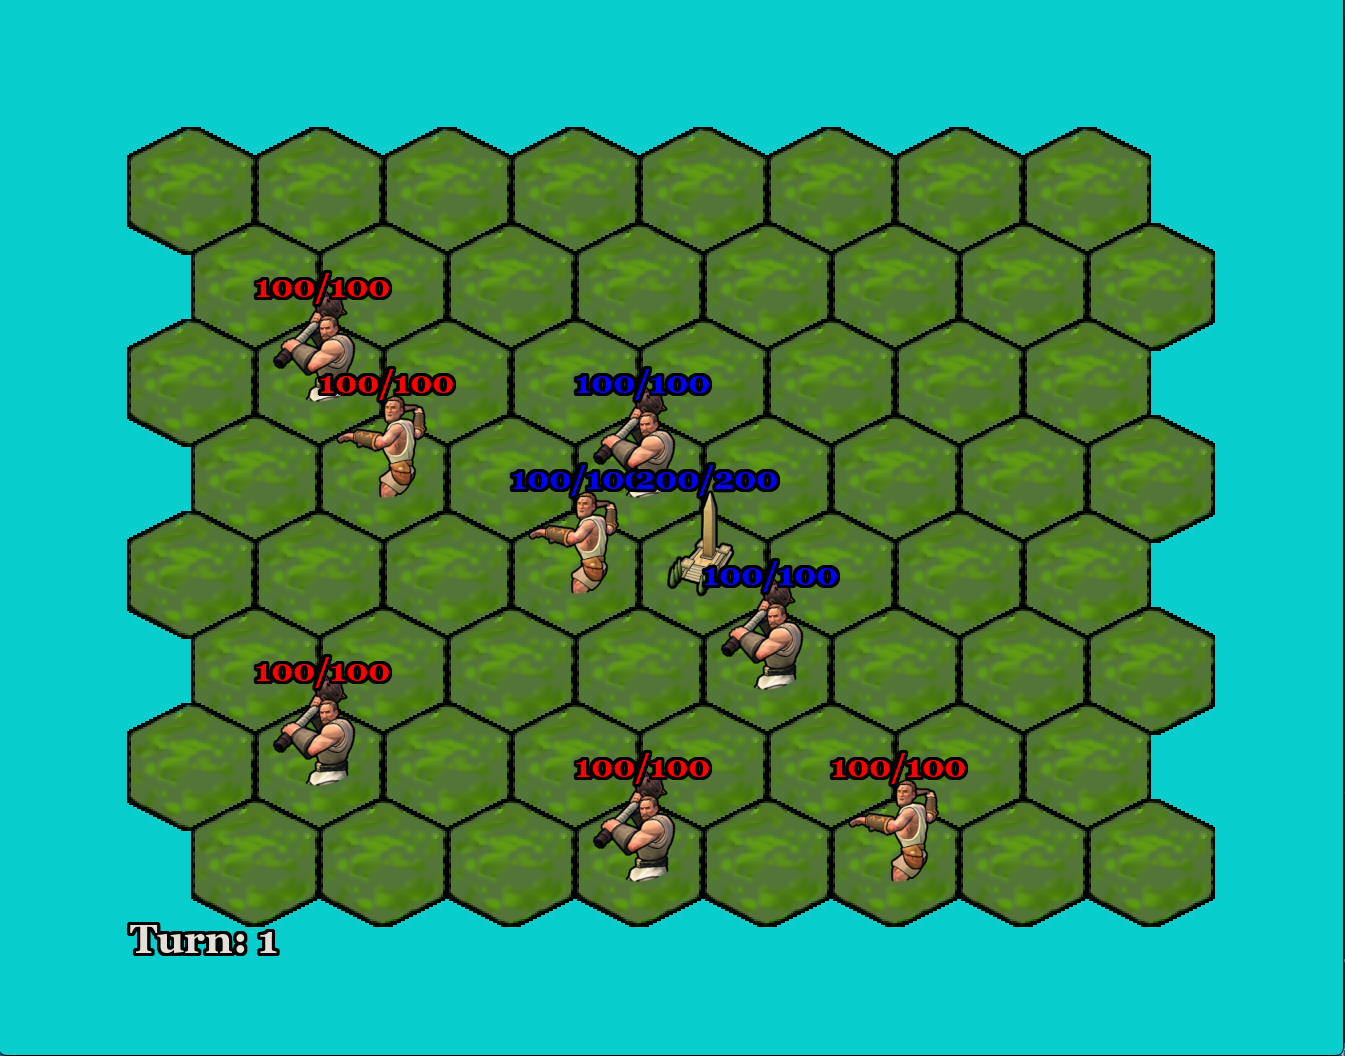
\includegraphics[scale=0.3]{gambar/environment_screenshot.png}
    % Keterangan gambar yang diinputkan
    \caption{\emph{Screenshot environment} dalam mode \emph{render}. \emph{Unit} milik agen \emph{attacker} memiliki teks \emph{hit points} berwarna merah dan unit milik agen \emph{defender} memiliki teks \emph{hit points} berwarna biru.}
    % Label referensi dari gambar yang diinputkan
    \label{fig:environmentScreenshot}
\end{figure}

\subsection{Unit dan Kota}
\emph{Unit} yang paling banyak jumlahnya dalam \emph{environment} ini adalah \emph{warrior}. 
\emph{Warrior} merupakan \emph{melee unit}, yang mana hanya dapat menyerang lawan yang berada di sebelah unit tersebut.
\emph{Warrior} memiliki attribut sebagai berikut:
\begin{itemize}
  \item HP: 100
  \item \emph{Movement Points}: 2
  \item \emph{Combat Strength}: 20
\end{itemize}

Jenis \emph{Unit} kedua adalah \emph{slinger}. \emph{Slinger} merupakan \emph{ranged unit} yang memiliki jarak sejauh 1 lantai.
\emph{Slinger} dapat menyerang \emph{unit} lain yang berdekatan dengan \emph{slinger} tanpa menerima \emph{damage} balasan dari \emph{unit} yang diserang.
\emph{Slinger} memiliki attribut sebagai berikut:
\begin{itemize}
  \item HP: 100
  \item \emph{Movement Points}: 2
  \item \emph{Combat Strength}: 5
  \item \emph{Ranged Strength}: 15
\end{itemize}

Kota merupakan tujuan utama yang perlu dihancurkan oleh agen \emph{attacker}. 
Kota akan berusaha melakukan perbaikan pada gilirannya dengan menambahkan +20 HP jika HP yang dimilikinya kurang dari nilai maksimum.
Kota tidak dapat melakukan perbaikan jika terdapat minimal tiga \emph{melee unit} milik agen \emph{attacker}.
Berikut adalah attribut dari kota:
\begin{itemize}
  \item HP: 200
  \item \emph{Combat Strength}: 28
\end{itemize}

\begin{figure}[!htb]
  \begin{minipage}{0.32\textwidth}
    \centering
    
\includegraphics[width=\linewidth]{gambar/warrior_1.png}
    \caption{\emph{Unit warrior}}\label{Fig:warrior}
  \end{minipage}\hfill
  \begin{minipage}{0.32\textwidth}
    \centering
    
\includegraphics[width=\linewidth]{gambar/slinger_1.png}
    \caption{\emph{Unit slinger}}\label{Fig:slinger}
  \end{minipage}
  \begin{minipage}{0.32\textwidth}
    \centering
    
\includegraphics[width=\linewidth]{gambar/city.png}
    \caption{Kota}\label{Fig:kota}
  \end{minipage}
\end{figure}

\subsection{Giliran dan Pergerakan Unit Agen}
\emph{Environment} dimulai dengan giliran agen \emph{attacker}, dilanjutkan oleh giliran kota, dan kemudian
ke giliran agen \emph{defender} sebelum kembali ke agen \emph{attacker}.
Berikut diagram urutan giliran dalam \emph{environment} ini:

\begin{figure}[H]
  \centering
    % Nama dari file gambar yang diinputkan
    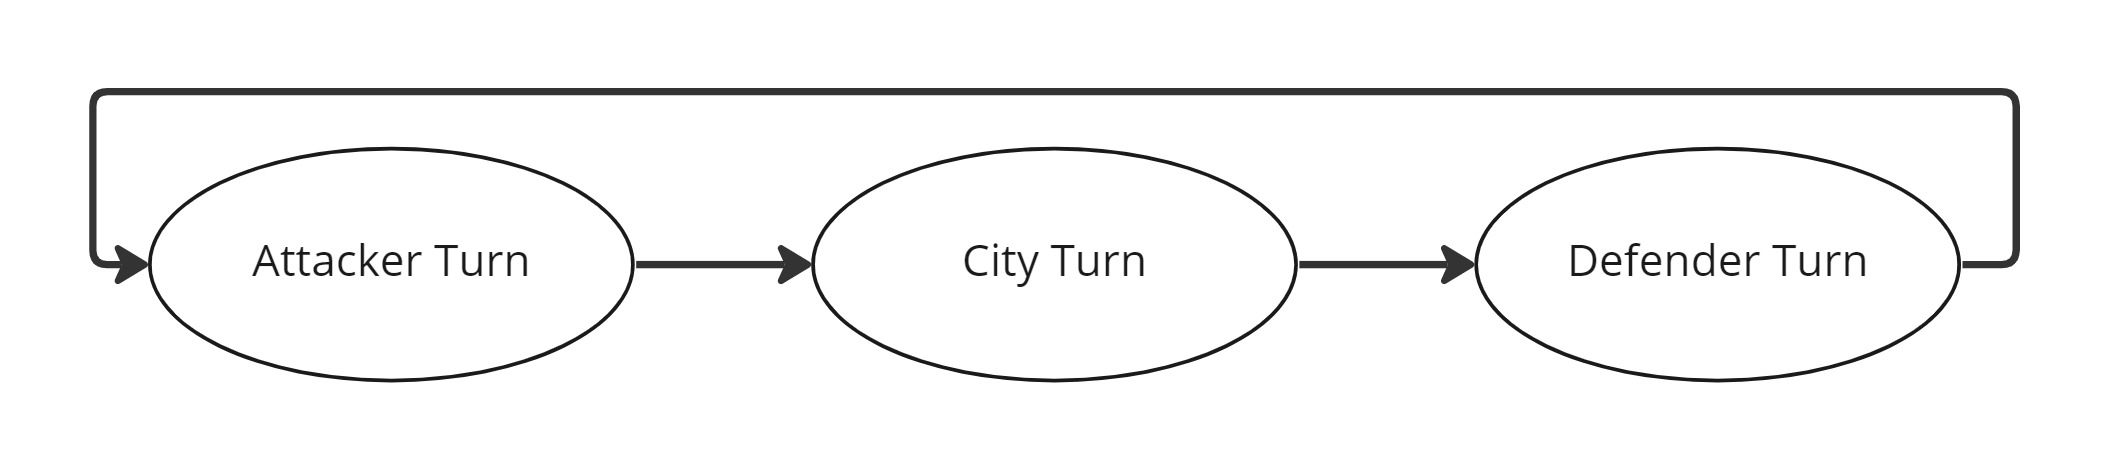
\includegraphics[scale=0.2]{gambar/turn_diagram.jpg}
    % Keterangan gambar yang diinputkan
    \caption{Diagram alur giliran agen}
    % Label referensi dari gambar yang diinputkan
    \label{fig:turnSequenceDiagram}
\end{figure}

Agen dapat mengkontrol \emph{unit} mereka pada giliran yang sudah ditentukan.
Pergerakan dan pemilihan \emph{unit} oleh agen dilakukan secara sekuensial. Pertama, agen akan memilih \emph{unit} pertama mereka.
Agen akan melakukan pergerakan dengan \emph{unit} yang telah dipilih sampai \emph{unit} tersebut tidak lagi memiliki \emph{movement points}
pada giliran tersebut.
Setelah itu, agen akan berpindah ke \emph{unit} selanjutnya. Hal ini akan berulang sampai agen tidak lagi memiliki unit yang masih
mempunyai \emph{movement points}. Jika agen sudah tidak memiliki \emph{unit} yang masih mempunyai \emph{movement points}
maka agen akan mengakhiri giliran mereka dan giliran berikutnya akan dimulai.
Berikut diagram dari pergerakan dan pemilihan sekuensial ini:

\begin{figure}[H]
  \centering
    % Nama dari file gambar yang diinputkan
    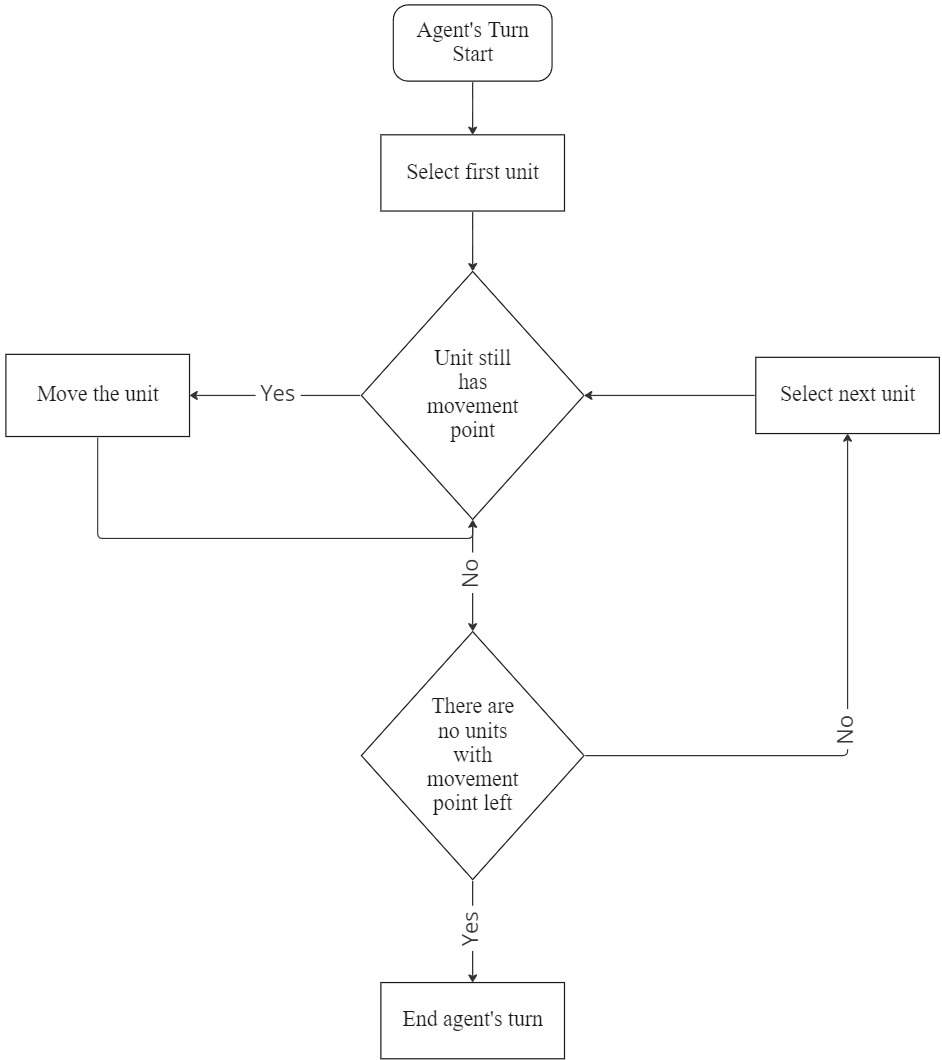
\includegraphics[scale=0.33]{gambar/unit_sequential_movement.jpg}
    % Keterangan gambar yang diinputkan
    \caption{Diagram pergerakan dan pemilihan sekuensial unit agen}
    % Label referensi dari gambar yang diinputkan
    \label{fig:sequentialMovementDiagram}
\end{figure}

Dalam giliran \emph{city}, jika tidak terdapat setidaknya tiga \emph{unit} agen \emph{attacker} didekat kota tersebut,
maka kota akan memulihkan 20 \emph{hit points} setiap gilirannya. Hal ini untuk mensimulasikan mekanisme keadaan \emph{siege}
dalam Civ6. Berikut diagram giliran pada kota:

\begin{figure}[H]
  \centering
    % Nama dari file gambar yang diinputkan
    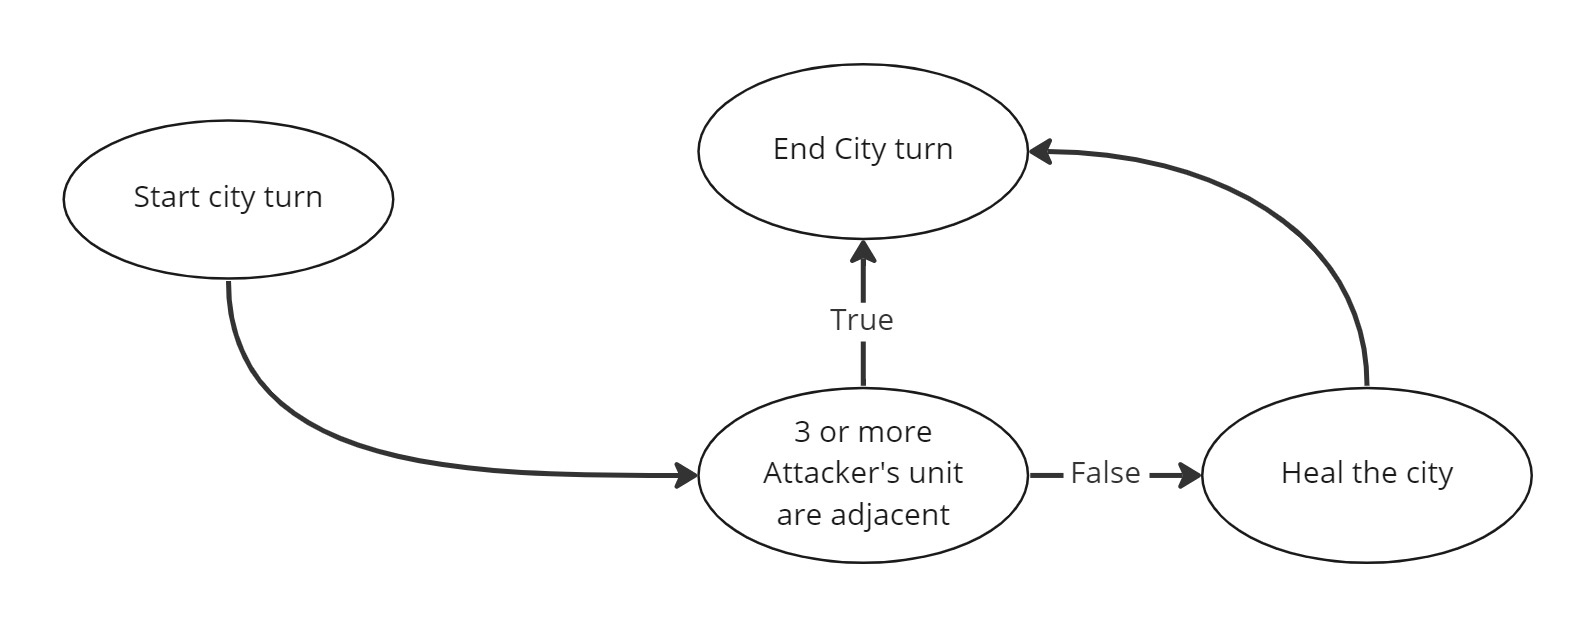
\includegraphics[scale=0.27]{gambar/city_turn.jpg}
    % Keterangan gambar yang diinputkan
    \caption{Diagram giliran kota}
    % Label referensi dari gambar yang diinputkan
    \label{fig:cityTurnDiagram}
\end{figure}

\subsection{Action Space}
\emph{Action space} merupakan kemungkinan yang dapat diambil oleh agen untuk melakukan sebuah \emph{action}.
\emph{Action space} yang digunakan dalam \emph{environment} ini adalah berupa 7 \emph{discrete actions}.
7 \emph{discrete actions} tersebut merupakan 6 sisi dimana \emph{unit} dapat bergerak ke dan 1 \emph{action} \emph{unit} tidak bergerak ke manapun.

% input gambar
\begin{figure}[H]
  \centering
    % Nama dari file gambar yang diinputkan
    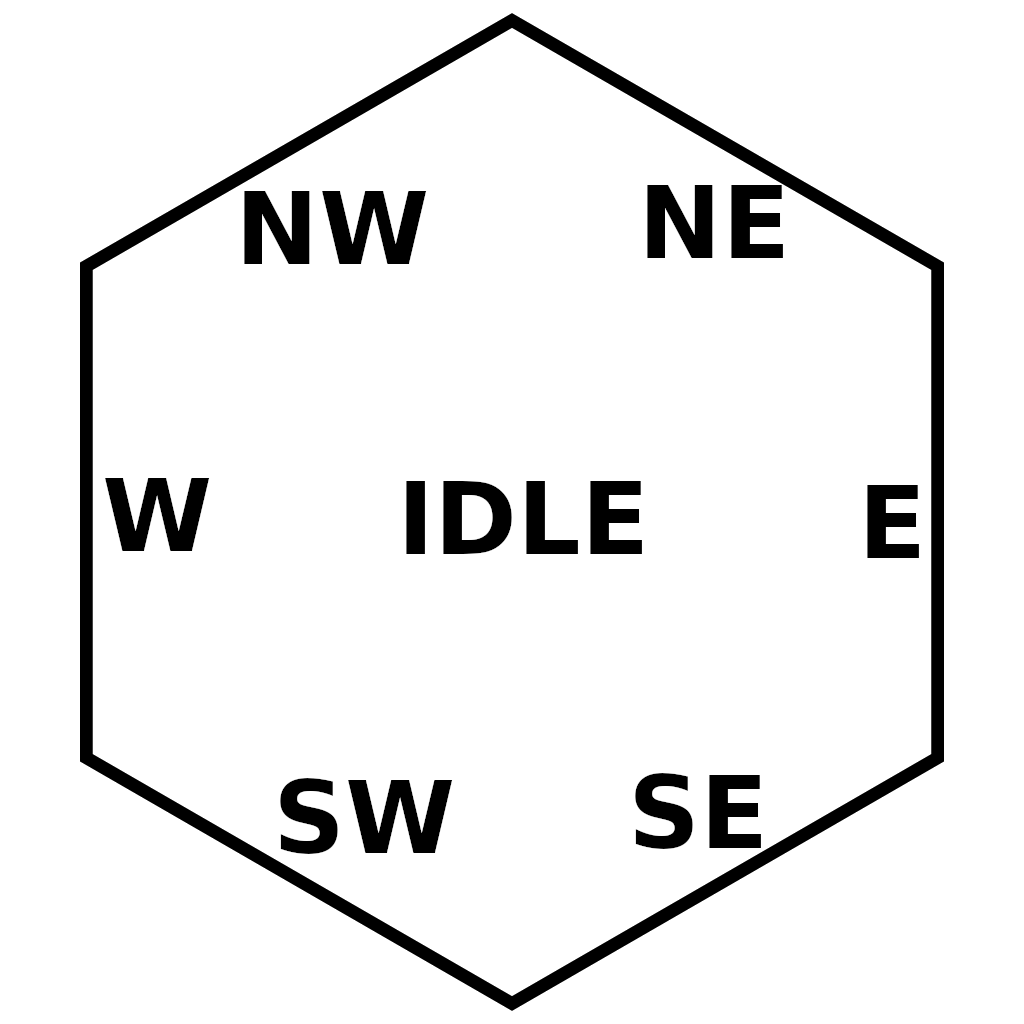
\includegraphics[scale=0.6]{gambar/hex_action.png}
    % Keterangan gambar yang diinputkan
    \caption{7 \emph{actions} yang dapat diambil oleh AI dalam \emph{Hexagonal tile}}
    % Label referensi dari gambar yang diinputkan
    \label{fig:hex_action}
\end{figure}

\emph{Unit} yang akan bergerak akan didapatkan nilai koordinat posisinya.
Dari koordinat posisi $y$ \emph{unit}, ditentukan paritas posisi \emph{unit}: apakah \emph{unit} berada dalam lantai genap atau ganjil.
\emph{Discrete actions} yang diberikan oleh agen kepada \emph{unit} kemudian akan diterjemahkan ke dalam koordinat lantai tujuan \emph{unit}.
Terjemahan \emph{discrete actions} yang diterima oleh \emph{unit}, mengikuti gambar \ref{fig:hex_action}:

\begin{itemize}
  \item 1: Bergerak ke NE
  \item 2: Bergerak ke E
  \item 3: Bergerak ke SE
  \item 4: Bergerak ke SW
  \item 5: Bergerak ke W
  \item 6: Bergerak ke NW
  \item 7: Diam di tempat (IDLE)
\end{itemize}

\subsection{Observation Space}
\emph{Observation Space} merupakan kumpulan \emph{state} dalam \emph{environment} yang didapatkan oleh agen saat melakukan observasi.
Agen dalam \emph{environment} penelitian ini melakukan \emph{complete observation}. 
Kedua agen mendapatkan informasi \emph{state} yang penuh dan sama saat melakukan observasi.
Seluruh nilai \emph{state} dinormalisasi sehingga nilainya berupa 0 sampai 1.
Berikut merupakan \emph{state} yang didapatkan oleh agen saat observasi:
\begin{itemize}
  \item Jarak seluruh \emph{unit} dari kota: $x_{1}, y_{1}, \dots x_{n}, y_{n}$
  \item Nilai HP dari seluruh \emph{unit}: $HP_{1}, \dots HP_{n}$
  \item Nilai movement points dari seluruh \emph{unit}: $MP_{1}, \dots MP_{n}$
\end{itemize}

\subsection{Reward Agen}
\emph{Reward} merupakan nilai yang diberikan kepada agen ketika agen tersebut melakukan sebuah \emph{action}.
Karena \emph{environment} pada penelitian ini merupakan \emph{asymmetric}, maka terdapat dua tipe \emph{reward}:
\emph{general rewards} dan \emph{attacker rewards}. 
\emph{General rewards} adalah tipe \emph{reward} yang diberikan ke agen \emph{attacker} dan \emph{defender}.
Sedangkan \emph{attacker rewards} hanya diberikan pada agen \emph{attacker}.
Berikut \emph{reward} tersebut:
\begin{itemize}
  \item General rewards: \begin{itemize}
      \item Bergerak ke luar batas \emph{environment} = -1
      \item Melakukan \emph{healing} pada sebuah \emph{unit} = +0.1
      \item Menyerang \emph{unit} lawan = +0.2
      \item Mematikan \emph{unit} lawan = +3
  \end{itemize}
  \item Attacker rewards: \begin{itemize}
      \item Menghancurkan kota = +20
      \item Menyerang kota = +0.5
      \item Kota melakukan perbaikan = -0.3
      \item Sebuah \emph{unit} mati = -1
      \item Sebuah giliran telah berlalu = -1
  \end{itemize}
\end{itemize}

Agen \emph{attacker} akan mendapatkan +20 poin ketika menghancurkan kota, karena itu merupakan tujuan utama dari agen \emph{attacker}.
Jika sebuah \emph{unit} agen \emph{attacker} mati atau sebuah giliran telah berlalu maka agen \emph{attacker} akan mendapatkan -1 point
Hal ini untuk memaksa agen \emph{attacker} agar menyelesaikan tujuannya secepat mungkin dan meminimalisir kehilangan \emph{unit}.

Agen \emph{defender} yang memiliki tujuan untuk mencoba mencegah agen \emph{attacker} mendapatkan +3 poin ketika sebuah \emph{unit}
agen \emph{attacker} mati. Tidak diberikan penalti pada agen \emph{defender} ketika \emph{unit} mereka mati karena pada eksperimen sebelumnya,
hal tersebut membuat agen \emph{defender} terlalu pasif. Kedua agen akan mendapatkan penalti ketika mencoba untuk menggerakan \emph{unit}
milik mereka keluar dari batas \emph{environment}.

\section{Implementasi Algoritma DRL}
Implementasi algoritma dalam penelitian ini menggunakan RLlib versi 2.0.0.
Kami menggunakan RLlib dengan alasan bahwa algoritma yang diimplementasikan dalam \emph{library} ini
merupakan \emph{open source} yang masih aktif dan memiliki banyak kontributor. 
Penggunaan library tersebut juga mengurangi akan adanya \emph{bug} jika dibandingkan dengan implementasi manual.
Alasan kedua adalah kemampuan RLlib untuk diintegrasikan dengan simulator eksternal seperti \emph{Unity3D}
dan \emph{game engine} lainnya \citep{rllibDocumentation}.
Mengingat bahwa manfaat dari penelitian ini adalah memberi contoh implementasi DRL
bagi \emph{game developer}.
Reproduksi akan hasil eksperimen dari penelitian juga akan dipermudah dengan 
menggunakan sebuah \emph{open source library} RL seperti RLlib.
Terdapat 4 algoritma SOTA DRL yang diimplementasikan dalam \emph{environment} dalam
eksperimen penelitian ini: DQN, APE-X DQN, PPO, IMPALA. 
Algoritma-algoritma tersebut dipilih karena mencakup beberapa bidang dari DRL seperti
\emph{policy based learning}, \emph{value based learning}, dan \emph{distributed learning}.
\emph{Hyperparameter} dari algoritma-algoritma tersebut mengikuti \emph{hyperparameter}
dasar yang diberikan secara \emph{default} oleh RLlib 2.0.0 dengan beberapa pengecualian:
\begin{itemize}
  \item num\_rollout\_workers: Mengatur akan jumlah instansi parallel training yang berjalan.
  angka 3 dipilih karena APE-X DQN menggunakan 2 CPU core setiap pada \emph{rollout\_workers}
  dan 2 core dasar. Dengan 3 \emph{rollout\_workers}, APE-X menggunakan seluruh 8 core dari i7 9700K
  secara penuh.

  \item multi\_agent: untuk membedakan \emph{policy}
  yang digunakan oleh agen \emph{attacker} dan \emph{defender}

  \item num\_env\_steps\_sampled: jumlah \emph{environment steps} yang dilakukan sebelum training selesai.
  Dipilih angka 10 juta karena jika melampaui angka ini, APE-X DQN akan menghabiskan lebih dari 32GB RAM.
  Kapasitas RAM yang terdapat pada spesifikasi hanya 32GB.
  
  \item num\_gpus: Digunakan satu GPU dalam training.
\end{itemize}

\begin{lstlisting}[
  language=Python,
  caption={Cuplikan kode setting config (hyperparameter)},
  label={lst:customHyperparameter}
]
config.multi_agent(

  policies={pid: (None, obs_space, act_space, {}) for pid in

            test_env.env.agents},

  policy_mapping_fn=(lambda agent_id, episode, **kwargs: agent_id),

  )  

config.num_gpus = 1
config.rollouts(num_rollout_workers=3)
    
\end{lstlisting}

Selain \emph{hyperparameter} yang sama (\emph{common-configs}), setiap algoritma memiliki \emph{hyperparameter}
tersendiri yang khusus untuk algoritma tersebut (\emph{specific-configs}).

\subsection{Implementasi DQN}
DQN yang digunakan dalam implementasi RLlib secara default adalah \emph{Double Dueling} DQN
dengan PER. \emph{Replay buffer} dikompres menggunakan LZ4 untuk mengurangi penggunaan memori.

\begin{figure}[H]
  \centering
    % Nama dari file gambar yang diinputkan
    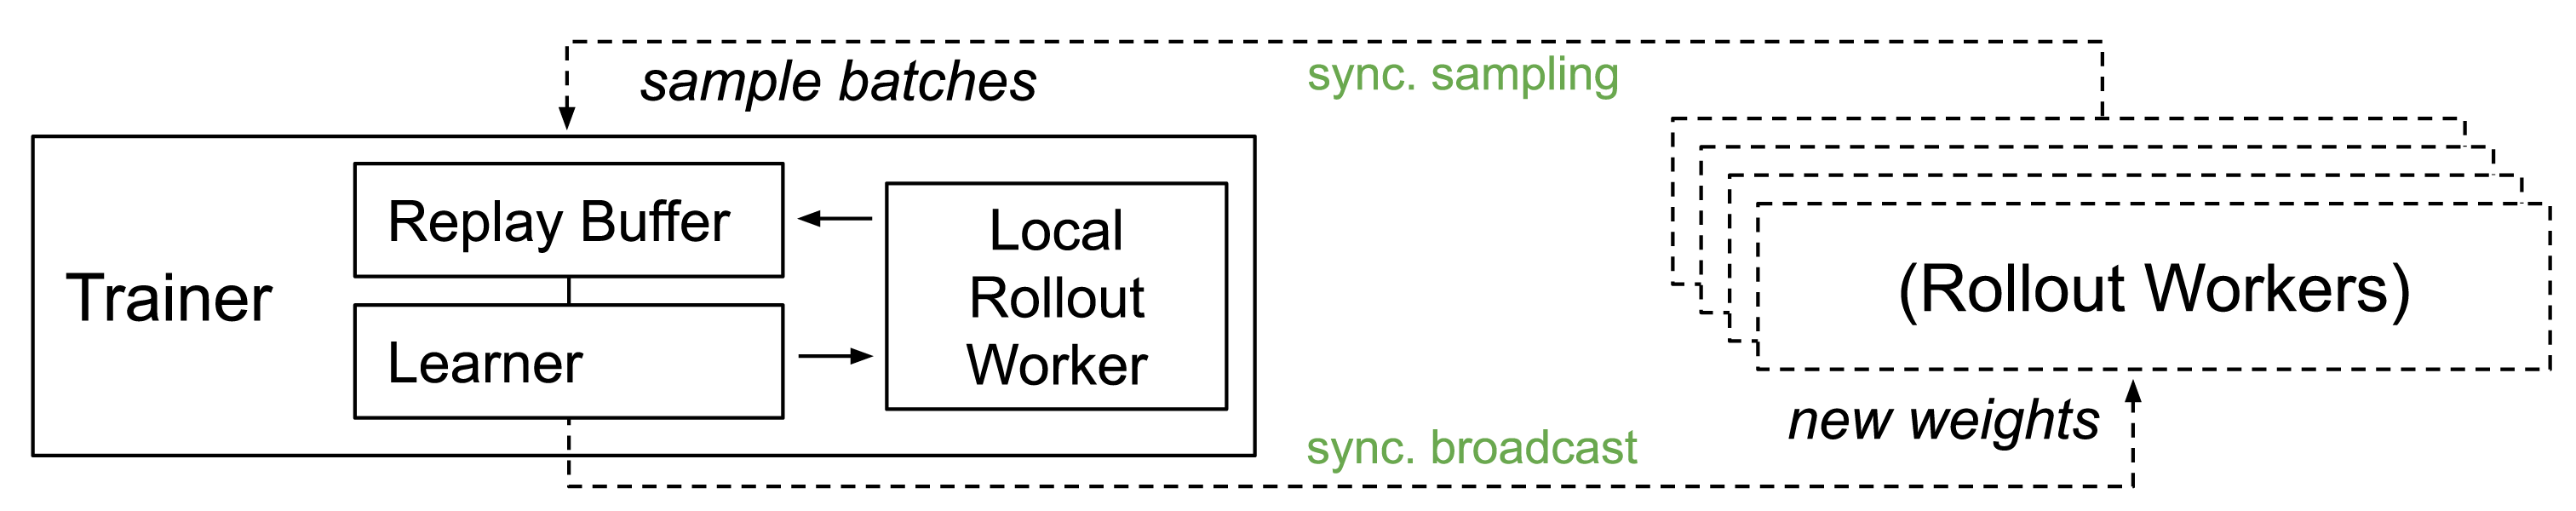
\includegraphics[scale=0.6]{gambar/rllib_dqn_architecture.png}
    % Keterangan gambar yang diinputkan
    \caption{Arsitektur DQN pada RLlib 2.0.0 \citep{rllibDocumentation}}
    % Label referensi dari gambar yang diinputkan
    \label{fig:rllib_dqn_architecture}
\end{figure}

\subsection{Implementasi APE-X DQN}
Implementasi APE-X DQN dalam RLlib 2.0.0 menggunakan implementasi DQN yang ada dengan
tambahan \emph{distributed prioritezed experience replay} (APE-X) untuk skalabilitas
yang mencapai ratusan CPU dengan satu GPU \emph{learner}. Pada \emph{specific-configs}
yang digunakan oleh APE-X DQN, digunakan 32 \emph{rollout\_workers}. Setting \emph{rollout\_workers}
tersebut terganti oleh 3 \emph{rollout\_workers} yang dideklarasikan pada \ref{lst:customHyperparameter}.

\begin{figure}[H]
  \centering
    % Nama dari file gambar yang diinputkan
    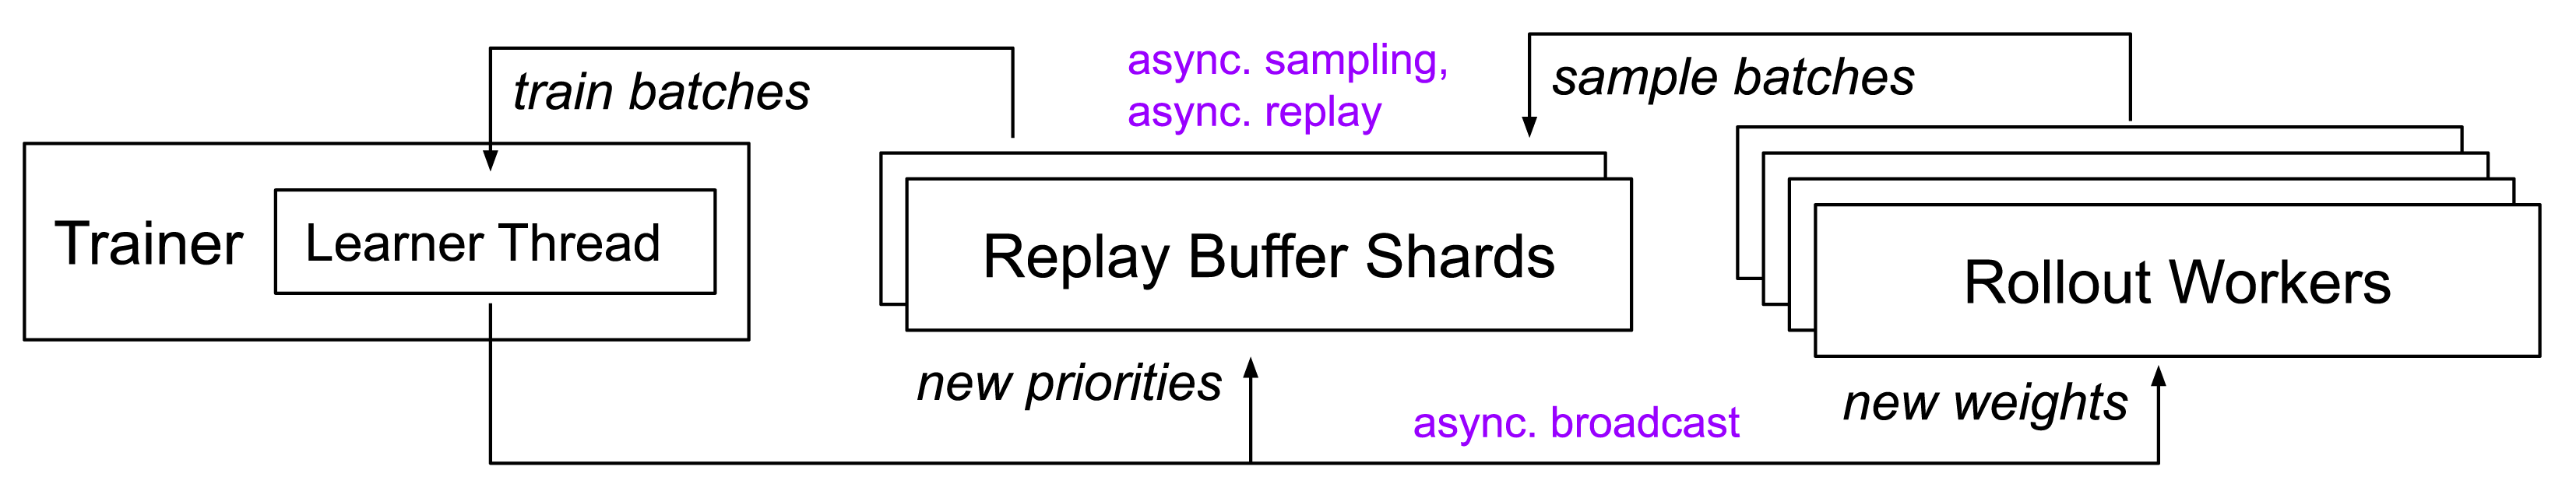
\includegraphics[scale=0.56]{gambar/rllib_apex-dqn_architecture.png}
    % Keterangan gambar yang diinputkan
    \caption{Arsitektur APE-X DQN pada RLlib 2.0.0 \citep{rllibDocumentation}}
    % Label referensi dari gambar yang diinputkan
    \label{fig:rllib_apex-dqn_architecture}
\end{figure}

\begin{figure}[H]
  \centering
    % Nama dari file gambar yang diinputkan
    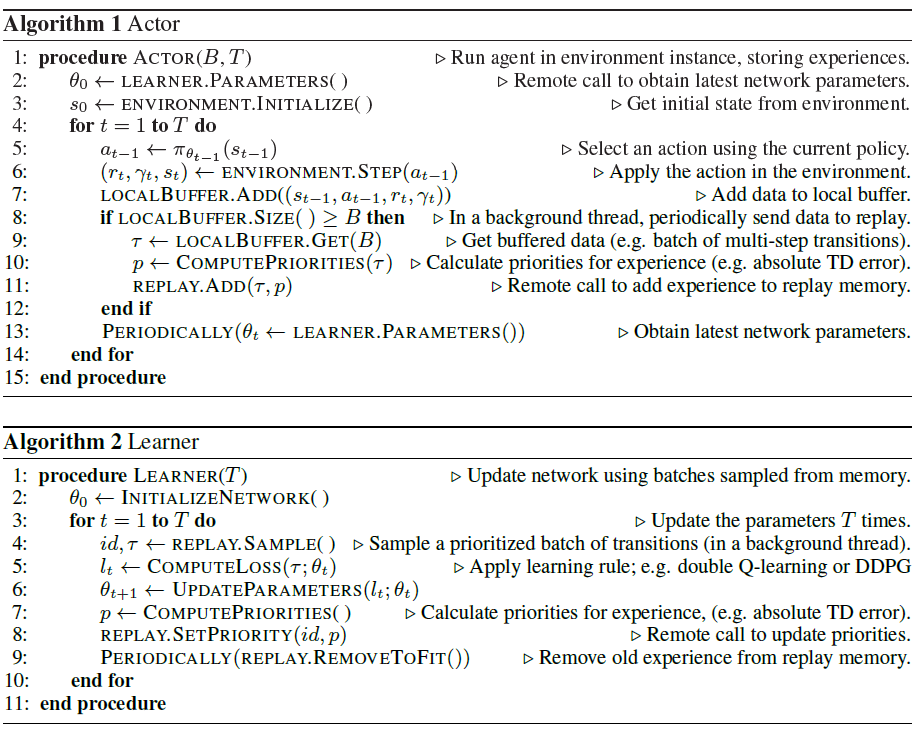
\includegraphics[scale=0.5]{gambar/apex_actor_learner_algorithm.png}
    % Keterangan gambar yang diinputkan
    \caption{Algoritma \emph{actor} dan \emph{learner} APEX DQN}
    % Label referensi dari gambar yang diinputkan
    \label{fig:apexActorLearnerAlgorithm}
\end{figure}

\subsection{Implementasi PPO}
Implementasi PPO dari RLlib 2.0.0 menggunakan \emph{clipped objective} dan \emph{KL-penalty}.
Multi-GPU \emph{optimizer} RLlib meletakkan data di GPU memori untuk menghindari transfer yang tidak diperlukan
dari \emph{host memory}, sehingga performa lebih baik dari implementasi secara \emph{naive}.

\begin{figure}[H]
  \centering
    % Nama dari file gambar yang diinputkan
    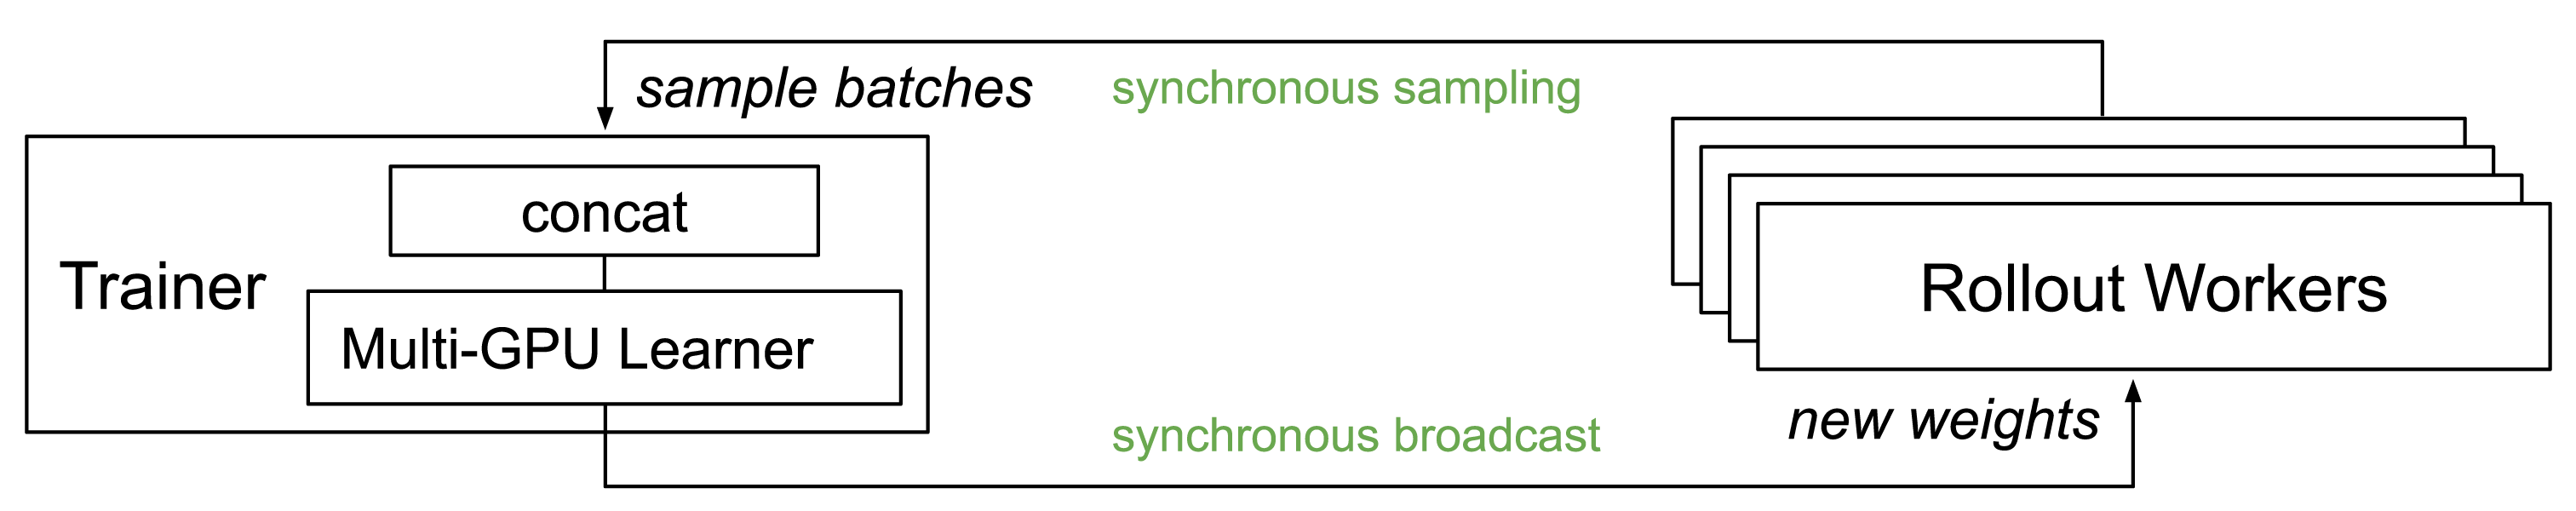
\includegraphics[scale=0.6]{gambar/rllib_ppo_architecture.png}
    % Keterangan gambar yang diinputkan
    \caption{Arsitektur PPO pada RLlib 2.0.0 \citep{rllibDocumentation}}
    % Label referensi dari gambar yang diinputkan
    \label{fig:rllib_ppo_architecture}
\end{figure}

\subsection{Implementasi IMPALA}
Implementasi IMPALA dari RLlib 2.0.0 menggunakan referensi kode V-trace milik DeepMind \citep{impala}.
Seperti APE-X DQN, IMPALA merupakan sebuah arsitektur terdistribusi. Arsitektur IMPALA juga mirip dengan PPO.
Akan tetapi, PPO menggunakan \emph{synchronous broadcast / sampling}, sedangkan IMPALA menggunakan \emph{asynchronous broadcast / sampling} dan \emph{replay buffer}.

\begin{figure}[H]
  \centering
    % Nama dari file gambar yang diinputkan
    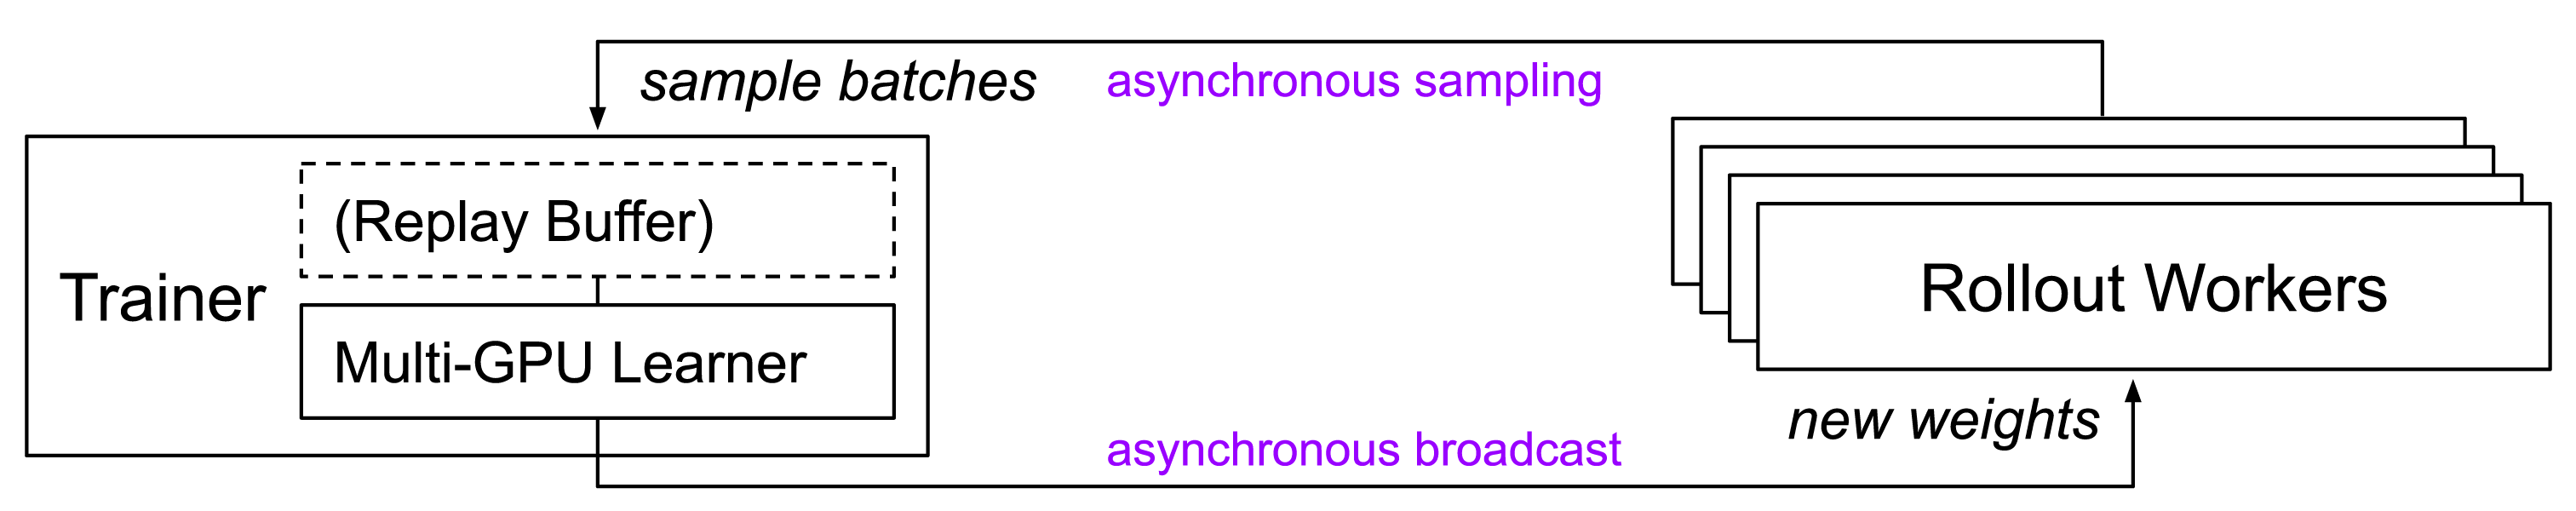
\includegraphics[scale=0.6]{gambar/rllib_impala_architecture.png}
    % Keterangan gambar yang diinputkan
    \caption{Arsitektur IMPALA pada RLlib 2.0.0 \citep{rllibDocumentation}}
    % Label referensi dari gambar yang diinputkan
    \label{fig:rllib_impala_architecture}
\end{figure}

\section{Tahap Eksperimen}
Dalam eksperimen, digunakan beberapa Tahap untuk \emph{training} dan \emph{testing} performa agen.
Tahap pertama adalah \emph{training}, dilanjutkan dengan evaluasi performa antar generasi agen, dan terakhir
evaluasi pada skenario \emph{environment} lebih besar.

\subsection{Training}
Training dilakukan dengan skenario \emph{environment} yang mengunggulkan agen \emph{attacker}.
Dalam skenario ini, agen \emph{attacker} memiliki jumlah \emph{unit} yang lebih banyak dari agen \emph{defender}.
Agen \emph{attacker} memiliki tiga \emph{unit} \emph{warrior} dan dua \emph{unit} \emph{slinger}.
Sedangkan agen \emph{defender} memiliki dua \emph{unit} \emph{warrior} dan satu \emph{unit} \emph{slinger}.
Dalam skenario ini, agen \emph{defender} diharapkan dapat menghancurkan kota secara konsisten, dengan keunggulan yang didapatkan oleh agen tersebut.

Performa agen \emph{attacker} juga akan lebih mudah dievaluasi dengan skenario ini.
Nilai \emph{reward} untuk menghancurkan kota memiliki nilai yang sangat besar: 20 poin, sehingga jika agen \emph{attacker}
dapat secara konsisten menghancurkan kota, nilai total \emph{reward} yang didapatkan akan jauh lebih banyak dibandingkan
jika agen \emph{attacker} gagal menghancurkan kota.

Setiap satu \emph{environment step}, sebuah agen melakukan satu pergerakan terhadap sebuah \emph{unit} miliknya.
Training dilakukan selama 100 juta \emph{total environment steps}.
Angka ini dipilih karena merupakan batas atas untuk menggunakan APEX DQN dengan spesifikasi PC ini.
APEX DQN akan membutuhkan RAM yang lebih dari 32GB ketika dijalankan lebih dari 100 juta \emph{total environment steps}.
Kami rasa, 100 juta \emph{total environment steps} juga lebih dari cukup untuk melakukan konvergensi pada seluruh algoritma
dalam \emph{environment} ini.

\begin{figure}[H]
  \centering
    % Nama dari file gambar yang diinputkan
    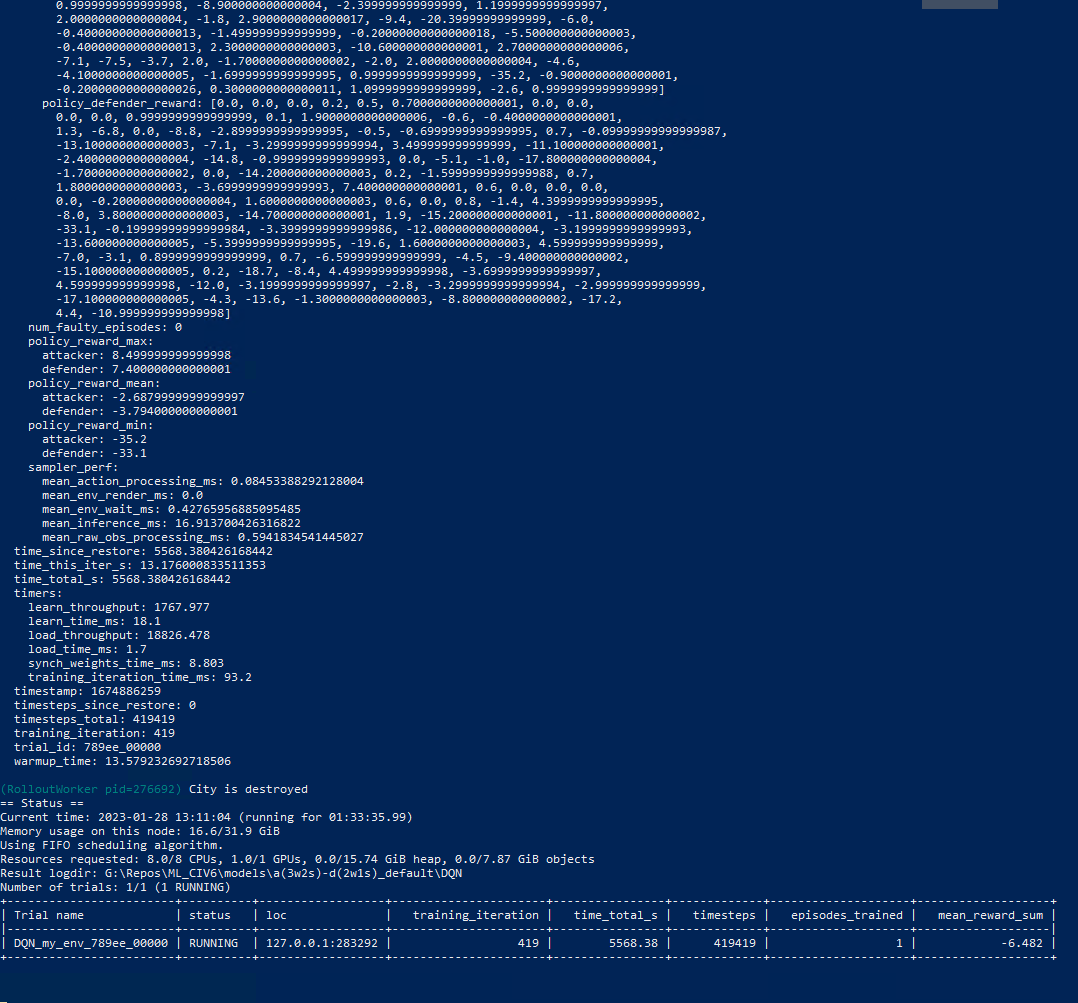
\includegraphics[scale=0.55]{gambar/training_process.png}
    % Keterangan gambar yang diinputkan
    \caption{Proses training pada algoritma DQN}
    % Label referensi dari gambar yang diinputkan
    \label{fig:trainingProcess}
\end{figure}

Hasil dari training ini merupakan beberapa generasi nilai bobot agen dari setiap algoritma dan nilai rata-rata \emph{rewards}
agen \emph{defender} dan \emph{attacker} dari setiap algoritma.
Nilai bobot beberapa generasi tersebut akan digunakan untuk proses evaluasi

\subsection{Evaluasi Antar Generasi Algoritma}
Didapatkan beberapa generasi yang dihasilkan selama proses \emph{training}. 
Dari generasi paling awal hingga generasi pada saat proses \emph{training} berakhir.
Secara umum, generasi yang paling akhir merupakan generasi yang memiliki performa paling baik.
Namun, tidak menutup kemungkinan adanya \emph{overfitting} yang terjadi pada generasi agen yang lebih akhir.

Pengujian antar generasi dilakukan selama 100 episode.
Dimana satu episode merupakan \emph{environment} yang sudah mencapai 20 giliran atau tujuan dari salah satu agen terpenuhi.
Generasi yang diambil merupakan 4 generasi yang dihasilkan dari training selama 10 juta \emph{total environment steps},
masing masing meliputi satu per empat bagian dari \emph{total environment steps} tersebut.
Hasil bobot disimpan berdasarkan iterasi \emph{training}.
Karena total iterasi \emph{training} setiap algoritma berbeda beda, maka berikut iterasi training yang diambil pada setiap algoritma:
\begin{itemize}
  \item DQN: iterasi 600, 1200, 1700, dan 2300
  \item APEX DQN: iterasi 100, 200, 300, dan 400
  \item PPO: 600, 1200, 1800, dan 2500s
  \item IMPALA: iterasi 200, 400, 600, dan 755
\end{itemize}

Evaluasi dilakukan secara urut. 
Dimulai dari generasi pertama agen \emph{attacker} melawan generasi pertama agen \emph{defender},
generasi pertama agen \emph{attacker} melawan generasi kedua agen \emph{defender}, 
dan seterusnya sampai generasi keempat agen \emph{attacker} melawan generasi keempat agen \emph{defender}.
Hasil dari evaluasi ini berupa nilai \emph{rewards} agen \emph{attacker} dan \emph{defender} dari setiap algoritma.

\subsection{Evaluasi dengan Environment Lebih Luas}
Untuk menguji adaptasi agen terhadap bentuk \emph{environment} lain, dilakukan evaluasi dengan skenario lain. 
Pengujian skenario dilakukan selama 100 episode untuk setiap generasi algoritma.
Skenario yang akan diujicobakan berukuran 16x16. 
Hasil dari pengujian adalah nilai \emph{reward} yang didapatkan oleh kedua agen pada setiap generasi.

\begin{figure}[H]
  \centering
    % Nama dari file gambar yang diinputkan
    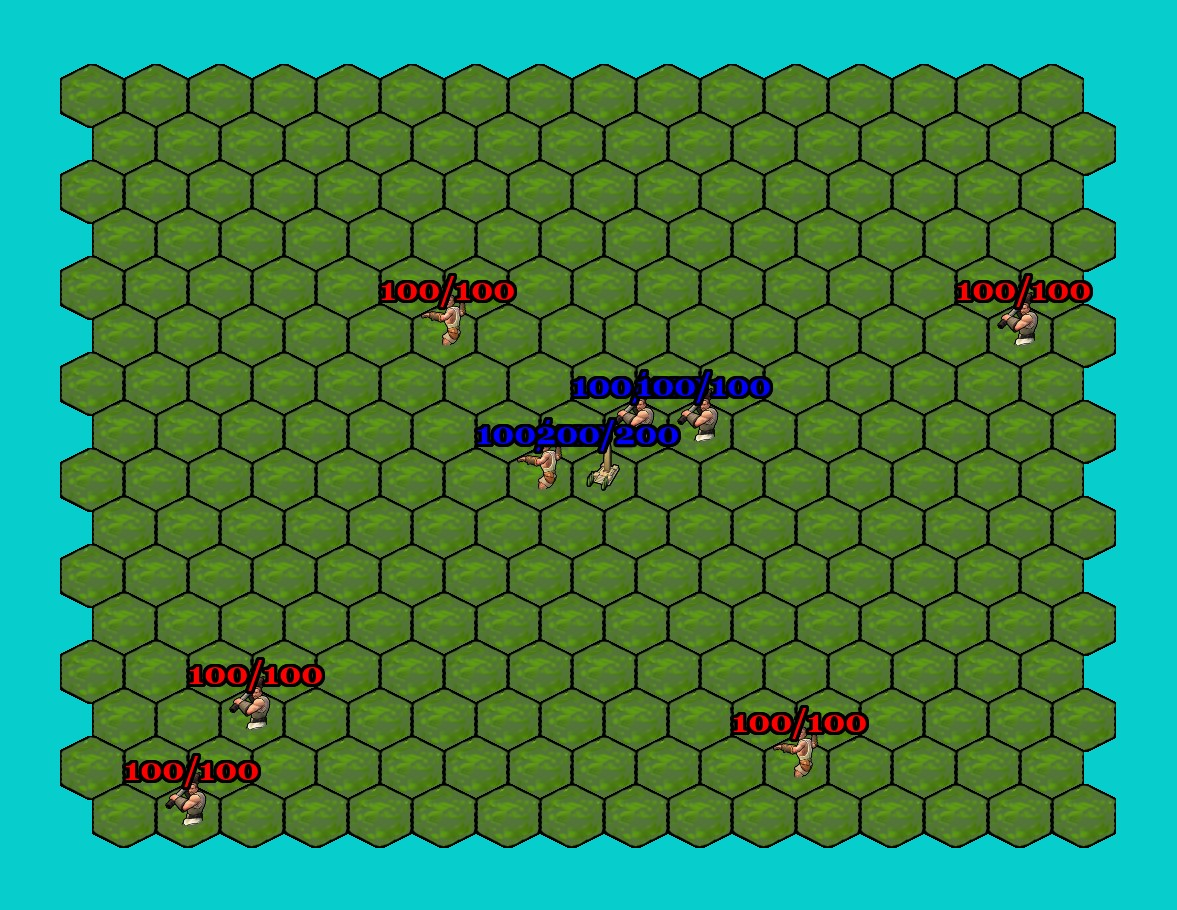
\includegraphics[scale=0.4]{gambar/16x16_env.jpg}
    % Keterangan gambar yang diinputkan
    \caption{\emph{Render environment} dengan ukuran 16x16.}
    % Label referensi dari gambar yang diinputkan
    \label{fig:16x16Environment}
\end{figure}